\section{Resultados}

Uno de los objetivos de la experimentación de este trabajo práctico era encontrar los mejores parámetros para los métodos, es decir, los parámetros para los cuales los algoritmos proporcionaban mejores resultados. Para determinar la calidad de los resultados obtenidos (cuáles eran los mejores) se tuvo en cuenta distintas métricas, que ayudaron a determinar esto mismo:

\begin{itemize}
\item Accuracy
\item F1-Score
\end{itemize}

Los resultados obtenidos fueron analizados en términos de estas métricas aplicando validación cruzada \textit{K-fold} (sobre la cual se hablará a continuación) sobre la base de entrenamiento.

Los parámetros $k$ (cantidad de vecinos en \textit{kNN}) y $\alpha$ (dimensión a la cual se reduce cada imagen con \textit{PCA}) fueron variándose como se expondrá en las páginas siguientes.

\subsection{K-fold}

La validación cruzada \textit{K-fold} consiste en particionar la base de entrenamiento en $K$ partes del mismo tamaño. Luego se realiza $K$ iteraciones, cada una de ellas reteniendo uno de los conjuntos para validación y utilizando los restantes $K - 1s$ para entrenamiento. Este método puede ser aleatorio, es decir, tomar las particiones sin cuidado alguno. Hicimos uso del método de MATLAB cvpartition, la cual tiene como define las particiones aleatoriamente de la cross-validation para un $n$ y un $K$.

\subsection{Tiempo de ejecución}

Medimos 2 cosas en términos de los tiempos de ejecución: el tiempo que toma realizar PCA sobre el set de entrenamiento, y el tiempo en aplicar kNN sobre uno de los elementos (incluyendo el cambio de base en el caso de haber realizado PCA).

Para estas mediciones tomamos los sets de entrenamiento y prueba provistos por la cátedra, correspondientes a la competencia de Kaggle. También usamos para estas pruebas $k = 10$ (para kNN) y $alpha = 100$ (para PCA). 

Los resultados fueron que, para el caso sin PCA, cada elemento de prueba tarda en promedio 500 ms en ser procesado. Consideramos que esto es relativamente lento, ya que al tratarse de 28,000 elementos, esto suma en total 3.89 horas, lo que resulta bastante prohibitivo y fue problemático a la hora de hacer experimentaciones.

En contraste, en el caso con PCA, cada elemento era procesado en aproximadamente 95ms, una mejora sustancial sobre todo considerando que esto incluye el cambio de base. Al aplicar sobre el set de prueba completo, esto demora alrededor de 45 minutos, una fracción del tiempo mencionado anteriormente.

Por último, cabe destacar que PCA en sí es un proceso costoso. Sin embargo, como nos esperábamos, el costo de PCA está compensado por las dimensiones de los sets utilizados, y aplicarlo sobre nuestro conjunto de entrenamiento demora en promedio 26 minutos, por lo que sumado a kNN, sigue representando apenas más del 25\% del tiempo de ejecución sin PCA.

Sin embargo, debe recordarse que el costo de PCA es elevado. Esto debe tenerse en cuenta junto con la precisión obtenida para sets de datos más pequeños, ya que podría no justificarse.

\subsection{K de kNN}

Para analizar el comportamiento al cambiar el K de kNN fijamos alfa de PCA en 2 valores 15 y 30. Corrimos experimentos para distintos estos K: 1, 2, 3, 4, 5, 7, 8, 8, 10, 15, 20, 30.

Nuestra hipótesis previo a correr los experimentos fue que para $k$s chicos, la posibilidad de que nuestro vecino más cercano sea un outlier representando otro dígito son más altas y para los $k$s grandes, pensamos que los dígitos que se encuentran en las fronteras, osea que se parecen a otros dígitos, se verían perjudicadas ya que por como funciona knn, pordía ocurrir que el más cercano sea, por ejemplo, 5 pero todos los siguientes sean 2. Por lo tanto, supusimos que los $k$s intermedios serían los que mejor funcionarían.

Habiendo corrido los experimentos, el gráfico de accuracy generado fue el siguiente:

\begin{figure}[H]
    \begin{center}
      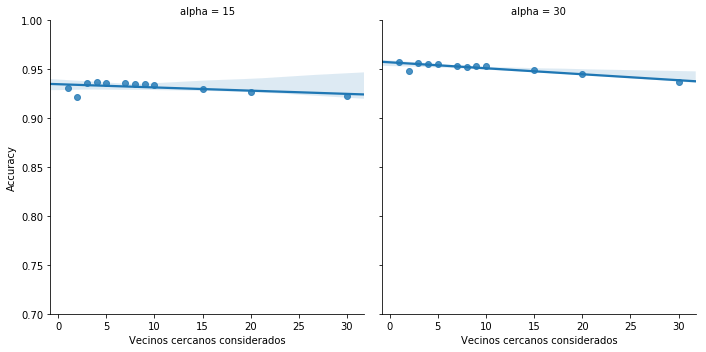
\includegraphics[width=0.8\columnwidth]{imagenes/Accuracy_15_30.png}
      \caption{Accuracy por k de kNN con alfa de PCA fijo}
    \end{center}
\end{figure}

Lo que se observó en este gráfico fue que el algoritmo es estable para los distintos $k$s y que las diferencias fueron poco significativas, pero pudimos contrastar con la hipótesis que lo que propusimos estaba en lo correcto.

El siguiente gráfico es una comparación del F1 score sobre los mismos resultados anteriores.

\begin{figure}[H]
    \begin{center}
      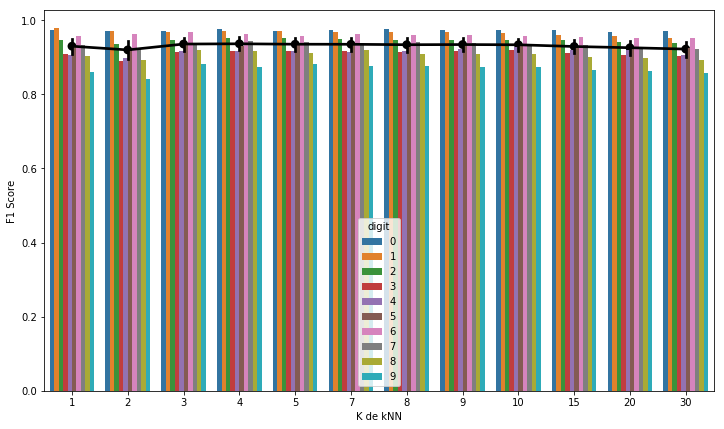
\includegraphics[width=0.8\columnwidth]{imagenes/F1_alpha_15.png}
      \caption{F1 score por k de kNN con alfa de PCA fijo en 15}
    \end{center}
\end{figure}

\begin{figure}[H]
    \begin{center}
      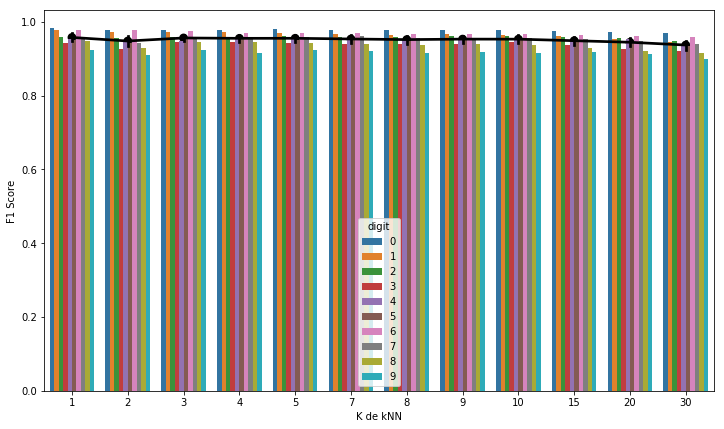
\includegraphics[width=0.8\columnwidth]{imagenes/F1_alpha_30.png}
      \caption{F1 score por k de kNN con alfa de PCA fijo en 30}
    \end{center}
\end{figure}

Este gráfico nos mostró también que el algoritmo es estable para cada dígito y que para alfa 30 de PCA las diferencias entre los dígitos es menor. En la siguiente sección entraremos en detalle sobre la comparación que realizamos sobre el alfa de PCA.

\subsection{Alfa de PCA}

El otro parámetro que tratamos de optimizar fue el alfa de PCA, de una forma similar al K, fijamos este y fuimos cambiando el alfa, por suerte ya teníamos resultados sobre el K, así que decidimos fijarlo en 5. Los alfas con los que experimentamos fueron: 5, 10, 15, 20, 25, 30, 40, 50, 60, 80, 100, 150

Nuestra hipótesis para este experimento fue que si tomabamos un alfa bajo tendríamos bastante ruido y que para alfas grandes, al agregar tantas componentes, se daría menor importancia a los componentes mas relevantes por lo que perdería un poco de calidad de resultados ya que utilizar valores altos tiende a parecerse a sólo hacer kNN.

El siguiente gráfico muestra el accuracy para cada alfa evaluado.

\begin{figure}[H]
    \begin{center}
      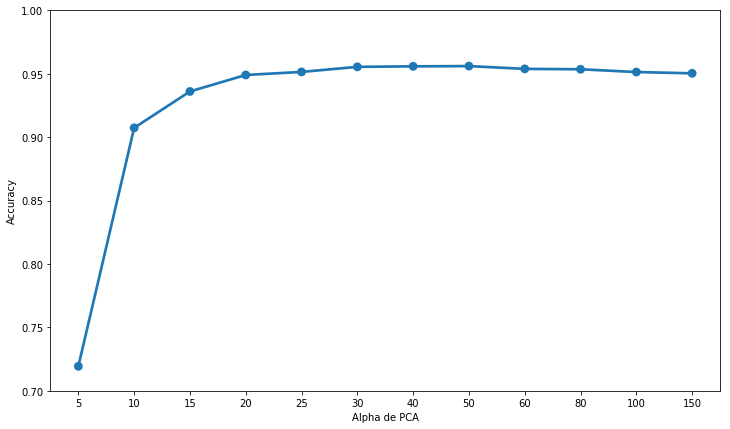
\includegraphics[width=0.8\columnwidth]{imagenes/Accuracy_all_alpha.png}
      \caption{Accuracy por alfa de PCA con k de kNN fijo en 5}
    \end{center}
\end{figure}

En este gráfico pudimos ver que los alfas que mejor funcionan de acuerdo al accuracy son los alfas entre 30 y 50 ya que a partir de ese momento es cuando el accuracy (lentamente) empieza a bajar.

El siguiente gráfico muestra F1 por dígito para cada alfa evaluado.

\begin{figure}[H]
    \begin{center}
      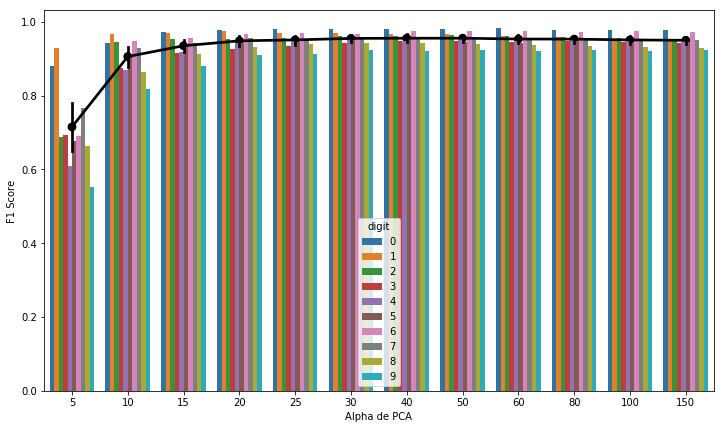
\includegraphics[width=0.8\columnwidth]{imagenes/F1_per_digit.png}
      \caption{F1 score por alfa de PCA con k de kNN fijo en 5}
    \end{center}
\end{figure}

En este caso se observó que para alfas muy bajos los resultados fueron bastante peores y que a medida que crece el alfa, se estabilizan más los resultados. 
Sabemos que a mayor alfa, más lento anda el algoritmo, por lo que podemos concluir que no es bueno tomar este tipo de valores dada la pequeña diferencia de calidad que hay entre ellos. Por eso decidimos que 30 era un buen alfa.

En base a estos experimentos concluímos que nuestra hipótesis era correcta, aunque esperábamos que para valores como 150 ande peor que lo que realmente funciona.

\subsection{Data augmentation}

Antes de entrenar el algoritmo con todo el dataset quisimos ver cómo el modelo de transformaciones escalaba, para eso corrimos sobre un subconjunto del set de datos, a los mismos 10k digitos les aplicamos la transformación para obtener así un dataset de 20k. Como ya teníamos el K y el alfa analizados usamos 5 y 30 respectivamente. Los resultados del experimento fueron una accuracy de 0.9602 para las rotaciones y de 0.9715 para las deformaciones elásticas. Pudimos apreciar una gran mejora con las deformaciones elásticas, esto se puede deber a que las rotaciones hay casos en los que no queda tan real el dígito generado.